% !TEX root = IROS2019_DNN.tex
\begin{section}{Run-time Verified Reachability for Safety} \label{sec:method}
\begin{figure*}[t]
	\centering
	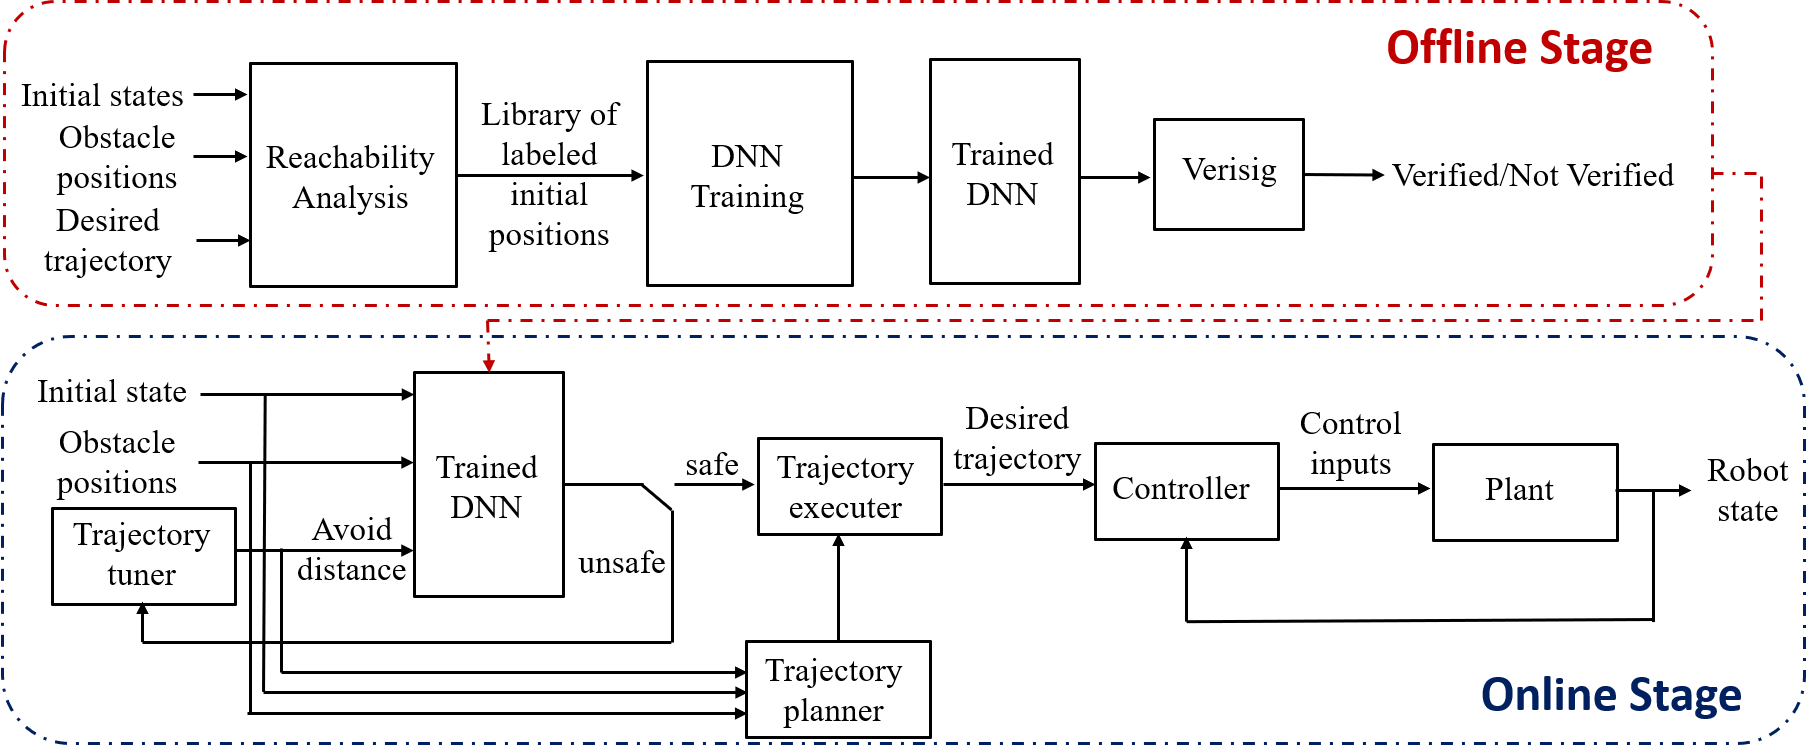
\includegraphics[width=0.8\textwidth]{figures/detailed_approach}
	\caption{Run-time verified reachability framework.}	
	\label{fig:det_app}
\end{figure*}

In this section, we describe our framework for run-time verified reachability for safety assurance of the autonomous operations. The proposed architecture is shown in Fig.~\ref{fig:det_app}.

In this work we propose a novel approach to make decisions about the safety of a trajectory at run-time using DNNs to predict the output of the reachability analysis in a very fast way. At the offline stage, obstacle free trajectories are generated from various initial positions to the given goal position. While designing the trajectory, the desired distance to keep from the obstacles (avoid distance) is specified by the user. Each initial position and avoid distance pair is labeled as safe or unsafe based on the reachability analysis. In this work, we use a simulation based reachability analysis for this particular system, however, the framework is independent from the choice of reachability tool. The aim is to predict the safety decisions of the reachability tool of choice in a fast way using DNNs. The library of labeled initial position-avoid distance pairs are used to train a DNN to predict the safety label of a different input pair. The trained DNN is then verified using Verisig and verified network is then used at online stage to make verified decisions about the safety of the trajectory from a given initial position to the goal position with a given avoid distance from the obstacles. 

The first step in our approach is the generate a trajectory library for offline training which is explained in the following section.
\subsection{Training Set Generation: Safety Labeled Initial Positions}
In order to have a network which is trained well enough to make accurate decisions, there is a need for a rich training set. In this work, the aim is to predict the safety of an initial position with a given avoid distance in a static environment. For this reason, a set of trajectories from a rich set of initial positions with different avoid distances is generated as explained in the following subsection.
\subsubsection{Trajectory Generation:}
In this work, trajectories are generated using minimum snap trajectories because of the fact that they are particularly suitable for quadrotor UAV dynamics to follow \cite{Mellinger2011}. We use an heuristic approach to avoid the obstacles in the environment, however any path planning algorithm can be used for this purpose. When there is an obstacle along the way to the goal position, a waypoint is added to the path which is away from the obstacle by the specified avoid distance ($ r_a $). Then the trajectory is generated to visit all the waypoints and the final goal position by using minimum snap trajectory generation. In Fig.~\ref{fig:trajs}, some sample trajectories with different avoid distances are shown. In Fig.~\ref{fig:traj1_025} and \ref{fig:traj1_03}, the trajectory is generated from the same initial position $ \boldsymbol{p}_0 = [0.3, 0, 1] $ with $ r_a = 0.25 $ and $ r_a = 0.3 $ respectively. In this work, it is assumed that the trajectories are generated by following the same rules.
\begin{figure}[h]
	\centering
	\subfigure[$ r_a = 0.25 $\label{fig:traj1_025}]{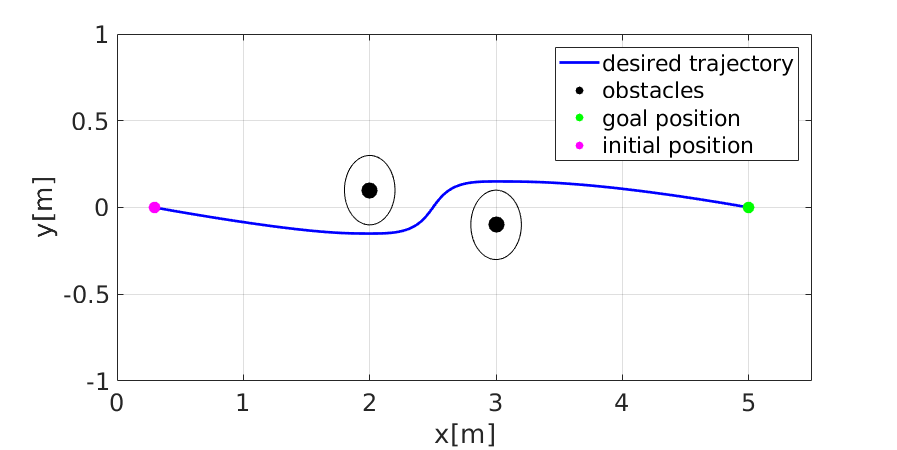
\includegraphics[width=0.22\textwidth]{figures/trajectories/traj_1}}
	\subfigure[$ r_a = 0.3 $\label{fig:traj1_03}]{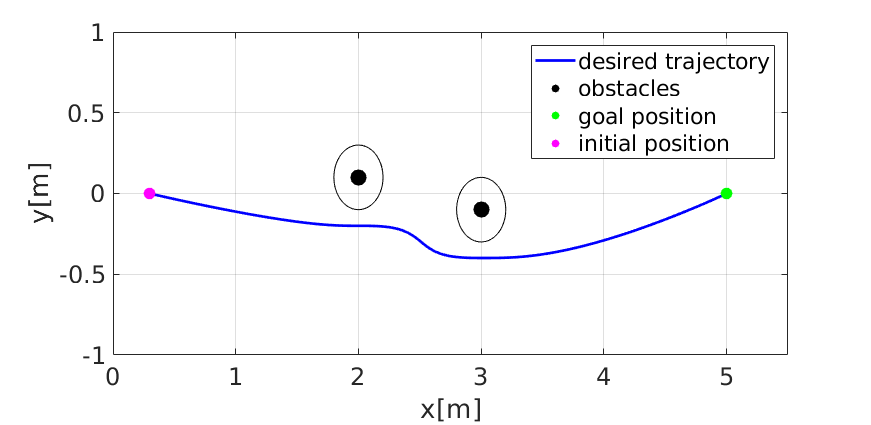
\includegraphics[width=0.22\textwidth]{figures/trajectories/traj_1_03}}
	%\subfigure[$ r_a = 0.25 $\label{fig:traj2_025}]{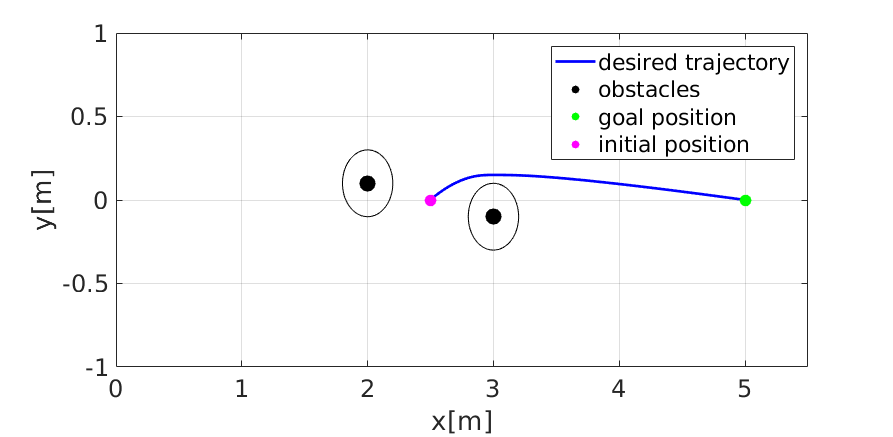
\includegraphics[width=0.22\textwidth]{figures/trajectories/traj_2}}
	%\subfigure[$ r_a = 0.3 $\label{fig:traj2_03}]{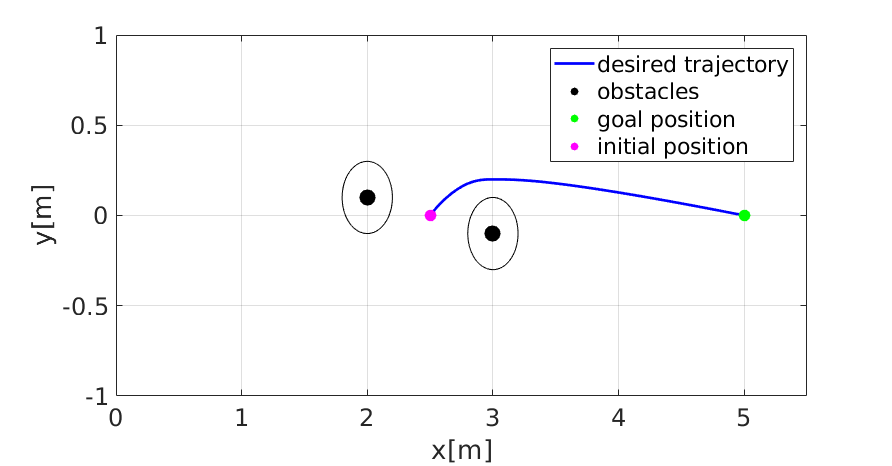
\includegraphics[width=0.22\textwidth]{figures/trajectories/traj_2_03}}
	\caption{Sample trajectories to avoid the obstacles with different avoid distances.}
	\label{fig:trajs}
\end{figure}

\subsubsection{Simulation-based Reachability Analysis:}
In order to decide if the trajectory from an initial position to the goal position is safe or not, reachability analysis needs to be performed on those trajectories. In this work, we use a simulation-based reachability analysis where the trajectories are run under the worst case scenario assumptions (i.e. worst disturbance in the environment). Under these assumptions, the maximum deviation from the trajectory at each time stamp is recorded ($ d_m(t) $). Since these maximum deviation values are recorded under worst case scenario assumptions, they can be used as upper bounds to the actual deviation from the trajectory. Then the position reachable sets are generated using as follows:
\begin{equation}
	\boldsymbol{R}(\boldsymbol{p}_\tau,t) = \{ \boldsymbol{p}(t): | \boldsymbol{p}(t) - \boldsymbol{p}_\tau(t) | \leq d_m(t) \}
	\label{eq:reach}
\end{equation}
In Fig.~\ref{fig:traj_reach}, the reachable sets generated for the trajectories in Fig.~\ref{fig:trajs} are presented.
\begin{figure}[h]
	\centering
	\subfigure[Reachable sets for the trajectory in Fig~\ref{fig:traj1_025}]{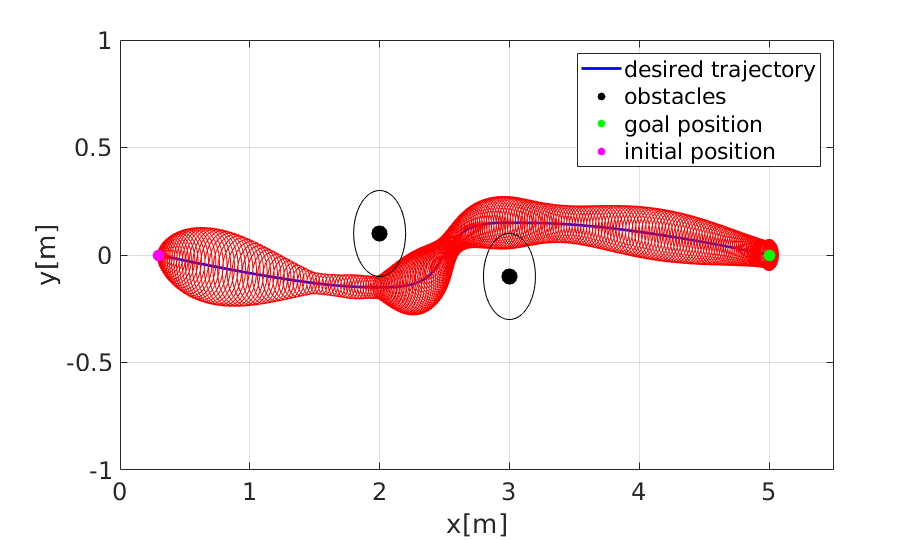
\includegraphics[width=0.22\textwidth]{figures/trajectories/traj_1_reach}}
	\subfigure[Reachable sets for the trajectory in Fig~\ref{fig:traj1_03}]{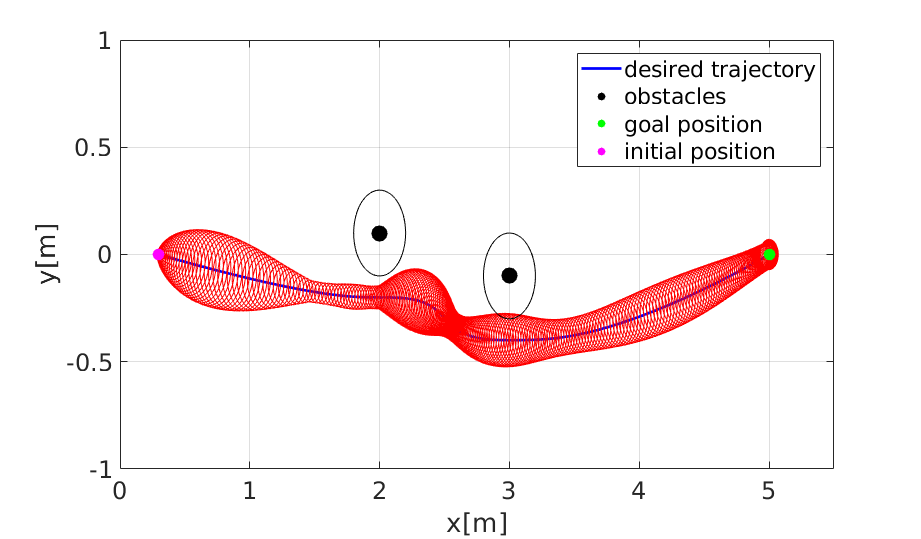
\includegraphics[width=0.22\textwidth]{figures/trajectories/traj_1_03_reach}}	
	\caption{Reachable sets for the trajectories in Fig.~\ref{fig:trajs}}
	\label{fig:traj_reach}
\end{figure}

The safety decision is made using these reachable sets. If the reachable sets of the trajectory are not intersecting with the obstacles, then the initial position and the avoid distance pair is labeled as safe:
\begin{equation}
	\begin{cases}
		s_{k,j} = 1 & \text{if   }  \boldsymbol{R}(\boldsymbol{p}_{\tau, k, j},t) \cap \boldsymbol{p}_{o,i} = \emptyset \\ 
		& \forall t \in [0,T], \forall i \in [1, \cdots, n_o], \\ 
		& k \in [1, \cdots, n_p], j \in  [1, \cdots, n_a] \\
		s_{i,j} = 0 & \text{otherwise}
 	\end{cases}
 	\label{eq:safety}
\end{equation}
where $ \boldsymbol{p}_{\tau,k,j} $ is the trajectory from $ k^{\text{th}} $ initial position with $ j^{\text{th}} $ avoid distance and $ s_{k,j} $ is the corresponding safety label. $ \boldsymbol{p}_o $ represents the $ o^\text{th} $ obstacle position, $ n_o $ is the number of obstacles in the environment, $ n_p $ is the number of initial positions in the training set and $ n_a $ is the number of different avoid distances in the training set. For instance, both trajectories in Fig.~\ref{fig:trajs} are labeled as unsafe since their reachable sets shown in Fig~\ref{fig:traj_reach} are colliding with obstacles.

In this work, we have generated a training set which includes 1886 initial positions whose $ x $ and $ y $ positions are uniformly distributed between $ [0,4.5] $m and $ [-2,2] $m respectively with $ 0.1 $m increments. During training six different avoid distances are used: $ r_a \in \{0.25, 0.3, 0.35, 0.4, 0.45, 0.5\} $. The entire training set consists of 11316 initial position-avoid distance pairs. In Fig~\ref{fig:safety_gt}, all the initial positions included in the training set are shown in the case environment. Safe initial positions are marked with green dots whereas unsafe initial positions are marked with red dots. For each avoid distance, a separate map is generated because the safety labels depend on the avoid distance as well. As can be noticed, as the avoid distance increases, number of safe initial positions also increases because the distance between the desired trajectories and obstacles becomes larger. Therefore, increasing avoid distance improves the safety, however the trajectories become longer, which is not something desirable for energy and time concerns.

\begin{figure}[H]
	\centering
	\subfigure[$ r_a = 0.25m $]{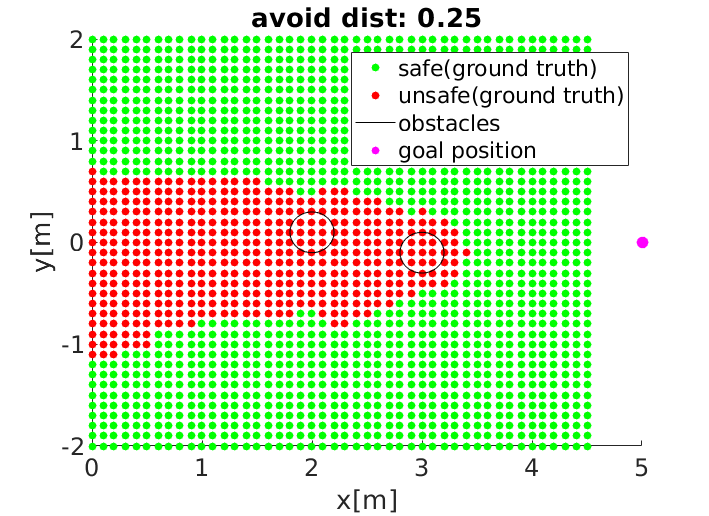
\includegraphics[width=0.15\textwidth]{figures/trajectories/training_gt_025}}
	\subfigure[$ r_a = 0.3m $]{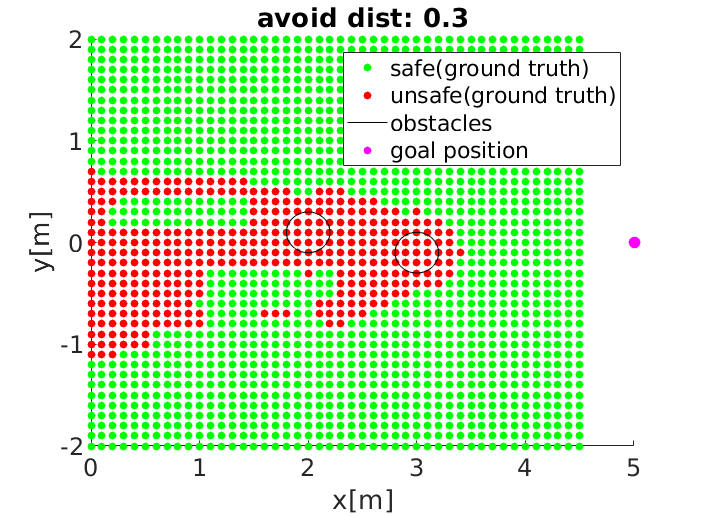
\includegraphics[width=0.15\textwidth]{figures/trajectories/training_gt_03}}
	\subfigure[$ r_a = 0.35m $]{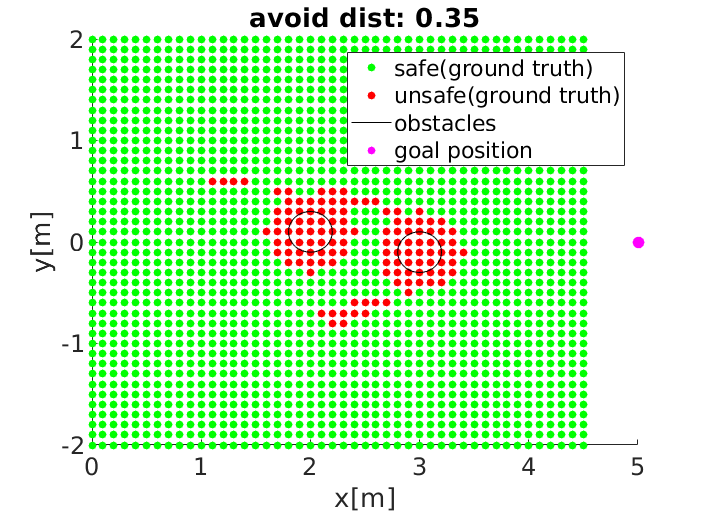
\includegraphics[width=0.15\textwidth]{figures/trajectories/training_gt_035}}
	\subfigure[$ r_a = 0.4m $]{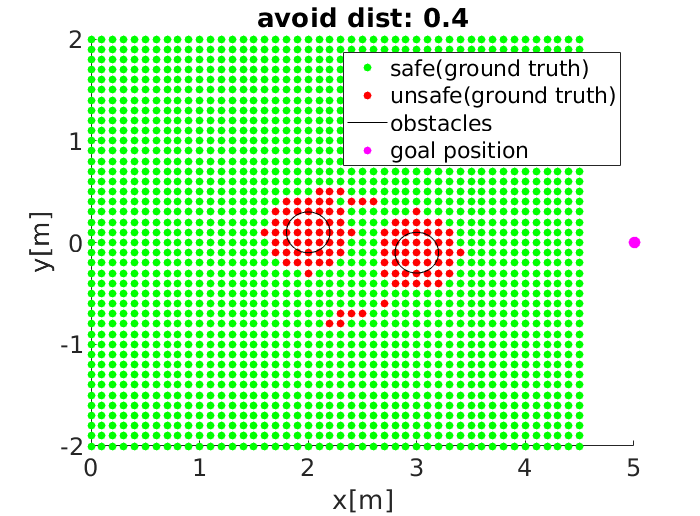
\includegraphics[width=0.15\textwidth]{figures/trajectories/training_gt_04}}
	\subfigure[$ r_a = 0.45m $]{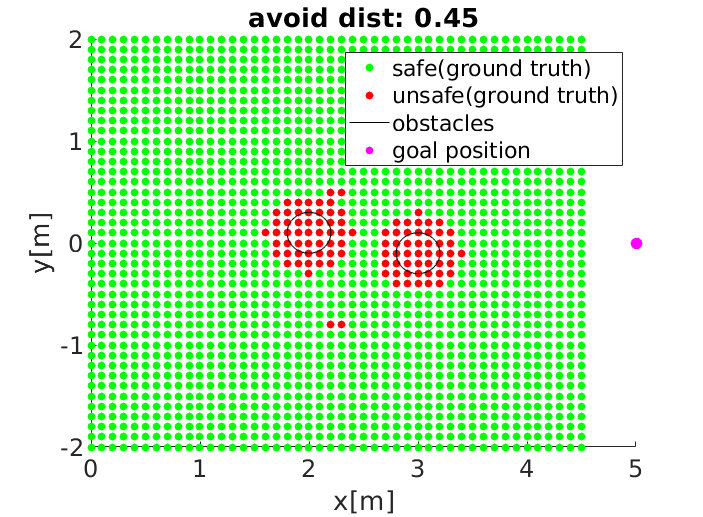
\includegraphics[width=0.15\textwidth]{figures/trajectories/training_gt_045}}
	\subfigure[$ r_a = 0.5m $]{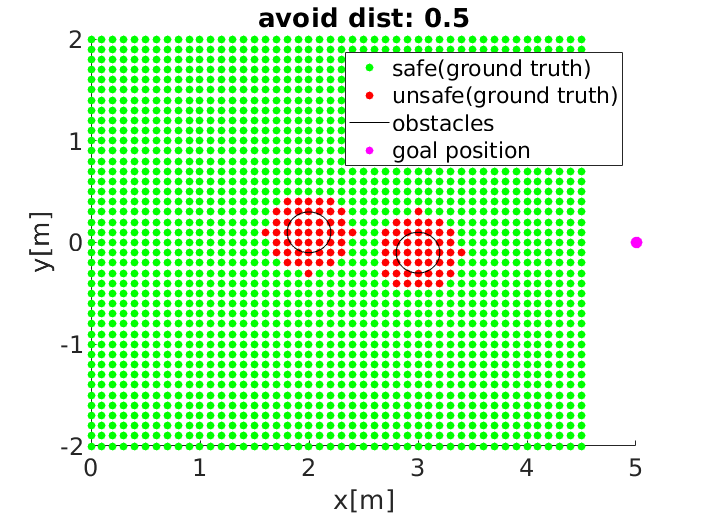
\includegraphics[width=0.15\textwidth]{figures/trajectories/training_gt_05}}
	\caption{Safety maps for the initial position in the training set with all avoid distances used in the training stage.}
	\label{fig:safety_gt}
\end{figure}

\subsection{Verified Reachability}
\subsubsection{DNN-Based Safety}
Neural networks have been used successfully in many application domains for recognizing patterns from a set of data. We are interested in classifying safe and unsafe trajectories given the initial position and the avoid distance radius.

We trained a shallow neural network (one hidden layer) with three node inputs, fifty hidden nodes, and two output nodes (one for each class).  
The network has been trained using the Neural Network Pattern Recognition Tool.
% using the standard 'trainfp' training function that has been shown to provide the best results for our training set. 
We decided to use only one hidden layer since the two classes are easy to discriminate concerning the inputs. Tests with more hidden layers (up to 50) have not shown consistent improvements. Multiple layers are in general more useful when more general features/concepts need to be classified.

Due to the high difference in the number of safe labels (~10k ) against unsafe ones (~1.2k), the training may result in returning false positive outputs (unsafe trajectory labeled safe). For this reason, we weight unsafe labels to be forty times more relevant than safe values. The training results showed 0\% False positive (FP) and around ~5\% False Negative (FN). The relatively high number of FN is more than acceptable since it is better to be over-conservative than being risky.
  
Fig.~\ref{fig:output_test} shows the output of the neural network when using the training set as input. Similarly to \ref{fig:safety_gt} each subfigure refers to a specific avoid distance radius. Dots represent the ground truth while circles the DNN output.
It is worth noting that, there are 0 FP values (red dots surrounded by green circles) while there is a certain number of FN (green dots surrounded by red circles) showing the conservative DNN behavior.
\begin{figure}[H]
	\centering
	\subfigure[$ r_a = 0.275m $]{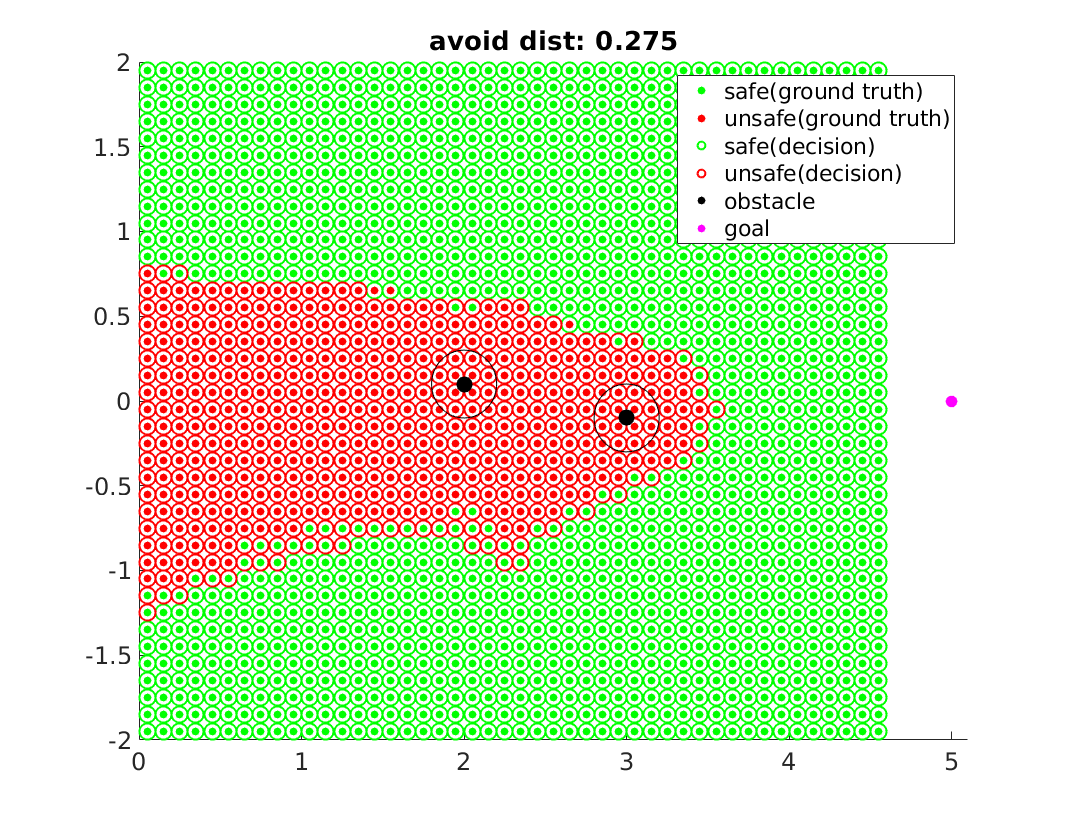
\includegraphics[width=0.15\textwidth]{figures/trajectories/testing_dec05_0275_new}}
	\subfigure[$ r_a = 0.3m $]{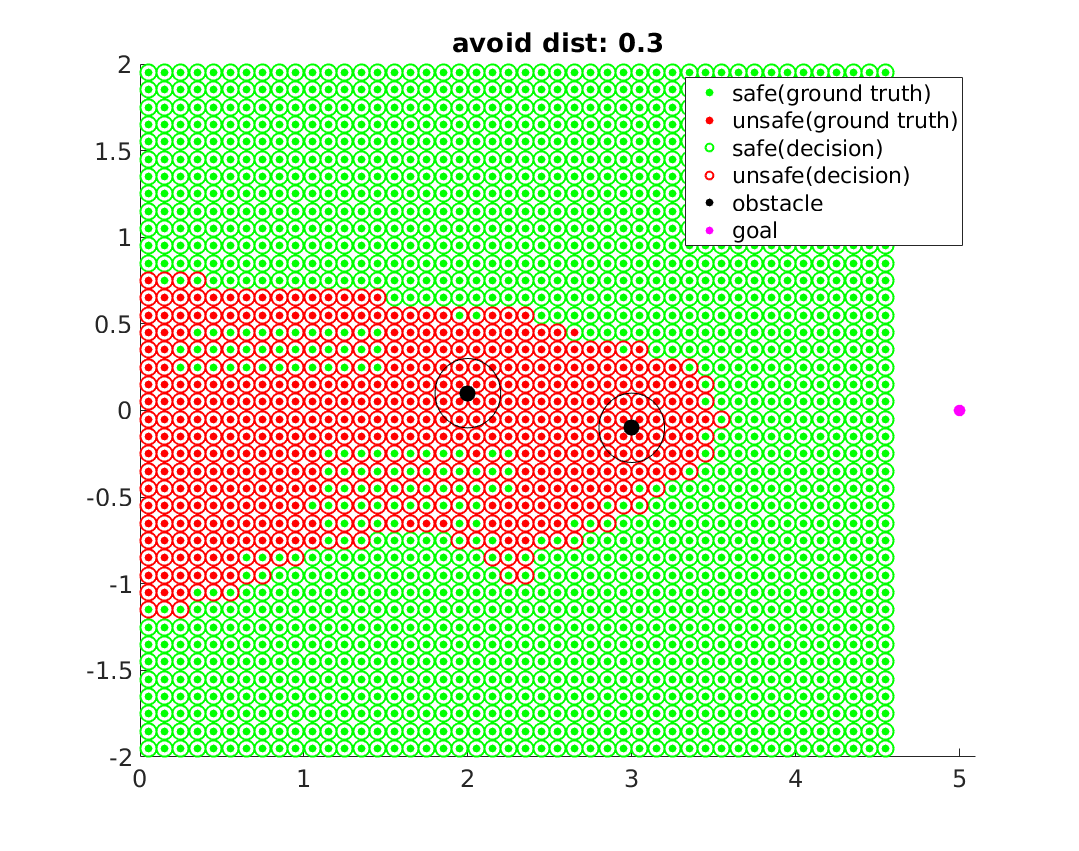
\includegraphics[width=0.15\textwidth]{figures/trajectories/testing_dec05_03_new}}
	\subfigure[$ r_a = 0.325m $]{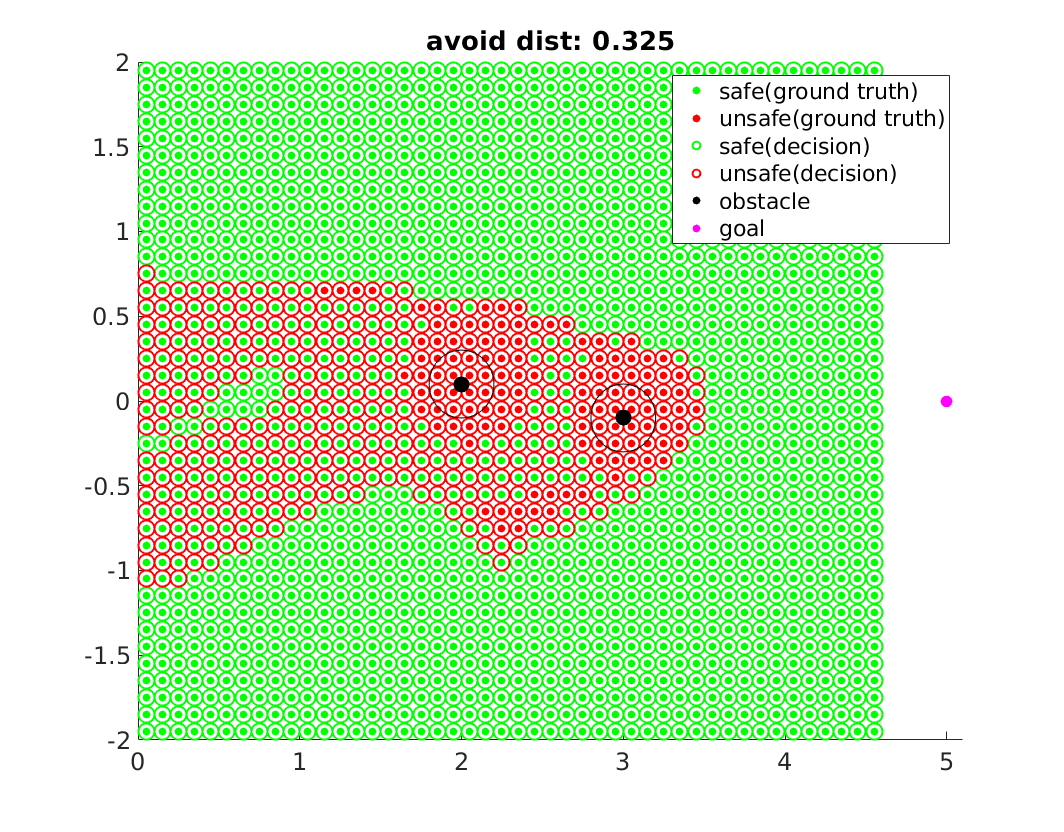
\includegraphics[width=0.15\textwidth]{figures/trajectories/testing_dec05_0325_new}}
	\subfigure[$ r_a = 0.375m $]{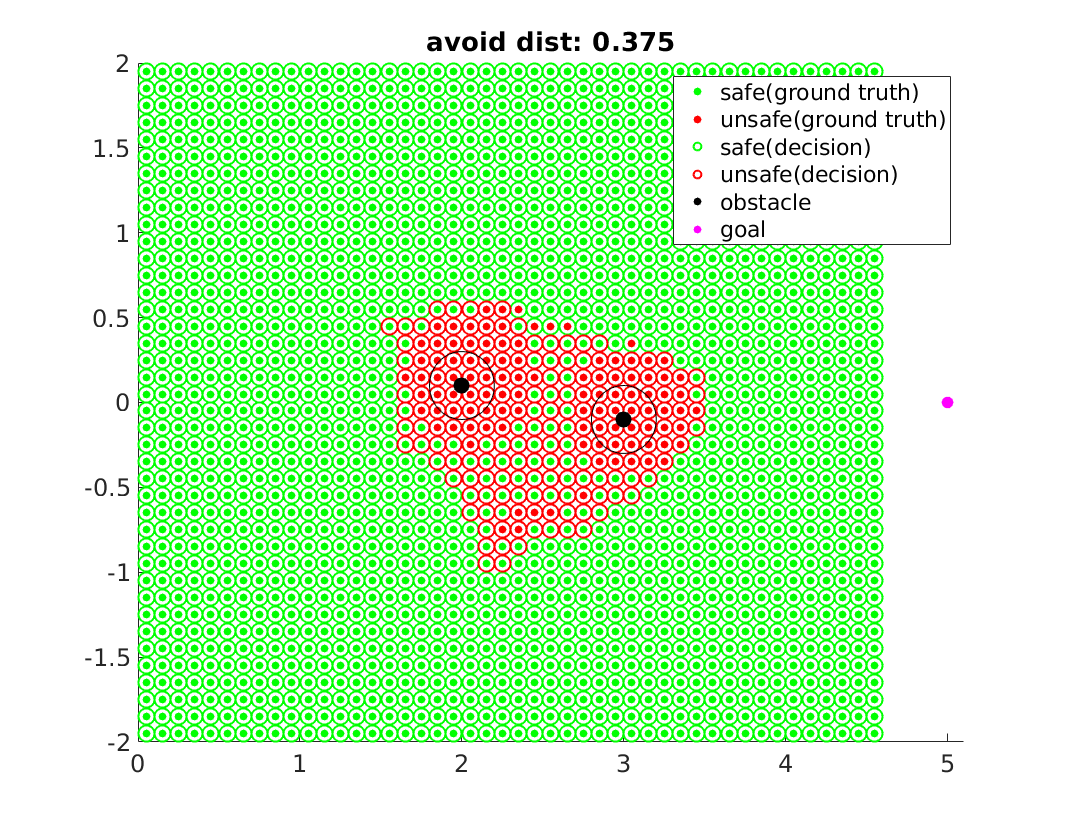
\includegraphics[width=0.15\textwidth]{figures/trajectories/testing_dec05_0375_new}}
	\subfigure[$ r_a = 0.425m $]{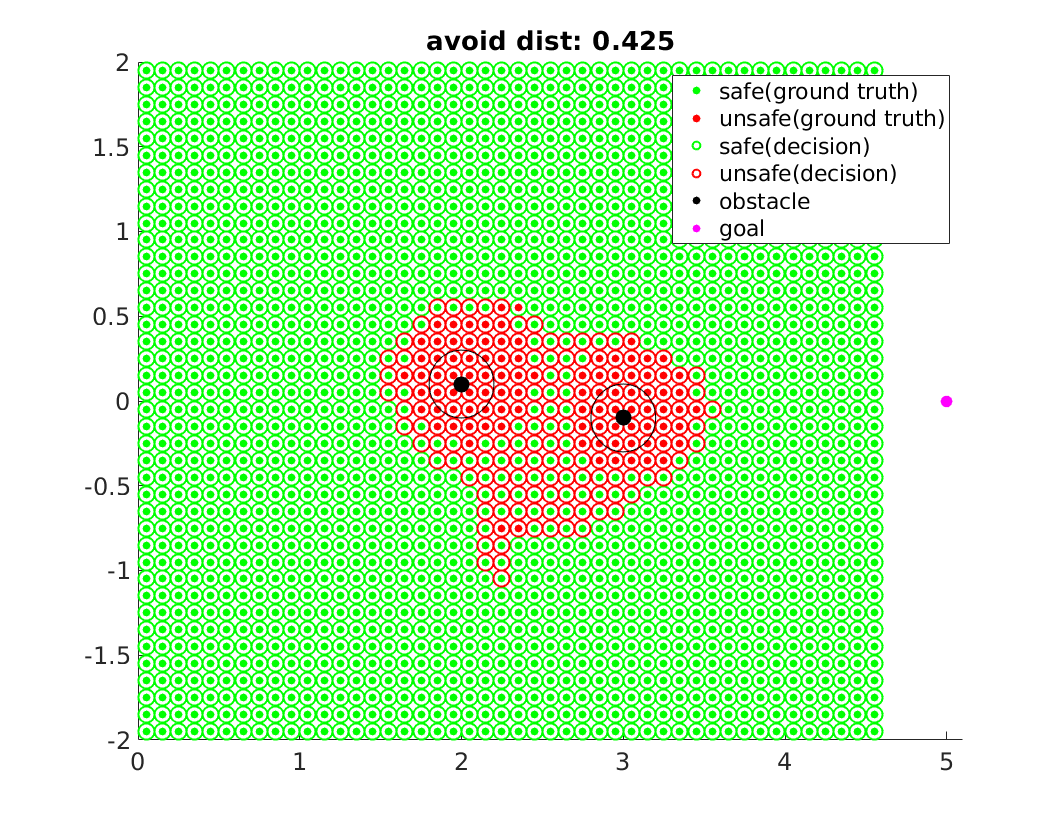
\includegraphics[width=0.15\textwidth]{figures/trajectories/testing_dec05_0425_new}}
	\subfigure[$ r_a = 0.475m $]{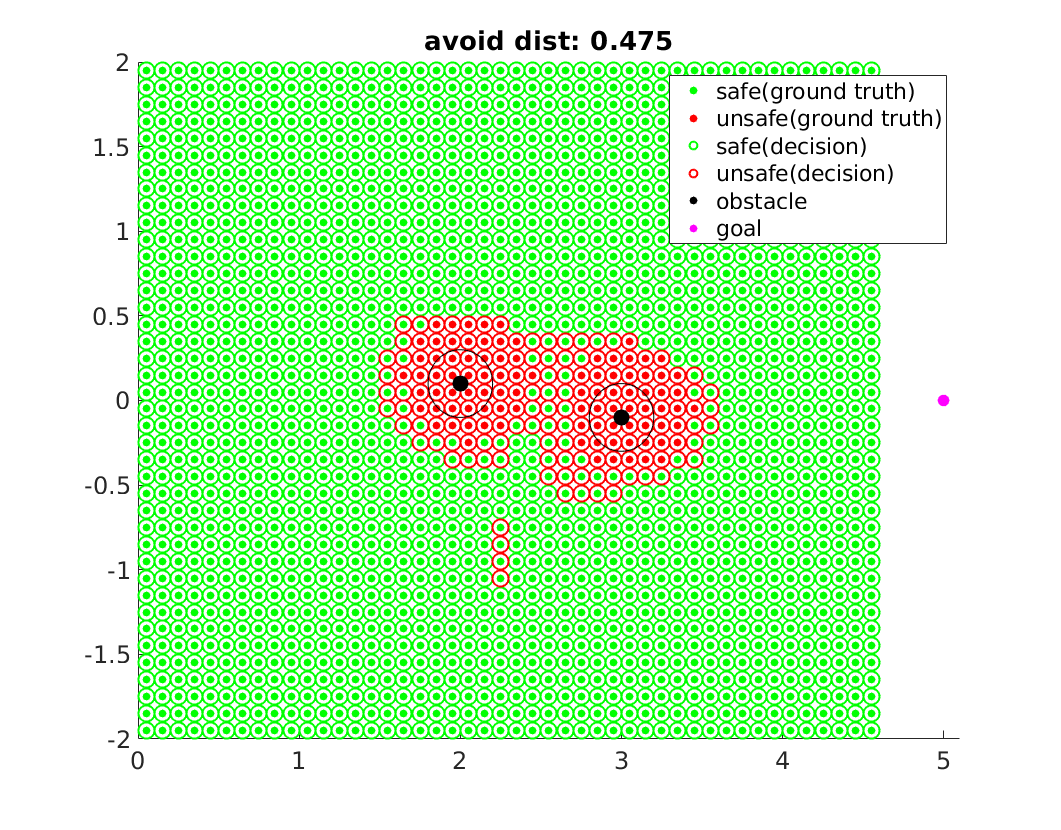
\includegraphics[width=0.15\textwidth]{figures/trajectories/testing_dec05_0475_new}}
	\label{fig:output_test}
	\caption{DNN safety decisions for test initial positions.}
\end{figure}

\subsubsection{Verisig}
Details about Verisig and how our network is verified (under what conditions) will be given here. \EY{I've left this out for now}

\end{section}
 